%%%%%
%
\section{Moyenne-Echantillonnage toutes fr�quences}

\itemstyle{Op�rateur~:} \operfmt{MoyEch\_ff}
\label{OP-MoyEch_ff}
\index{MoyEch\_ff}

%%%%%OBJET%%%%
\itemstyle{Objet~:}
Moyenne et �chantillonnage 
d'un param�tre � une fr�quence inf�rieure 
quelconque.

%%%%%ARGUMENTS%%%%
\bigskip
%%%%%ENTREES%%%%
\begin{tabarg}
\multicolumn{3}{l}{\titretab {Entr\'ees}}\\
\hline
$X$ & Vecteur, {\tt float} & Param\`etre d'entr\'ee \\
$f_{ei}$ & Coeff., {\tt float} & Fr\'equence d'\'echantillonnage de $X$\\
$f_{eo}$ & Coeff., {\tt float} & Fr\'equence d'\'echantillonnage de sortie\\
\end{tabarg}

\medskip
%%%%%SORTIES%%%%
\begin{tabarg}
\multicolumn{3}{l}{\titretab {Sorties}}\\
\hline
$X_m$ & Vecteur, {\tt float} & R\'esultat (m\^eme unit\'e que $X$)\\
\end{tabarg}


%%%%%FORMULE%%%%
\itemstyle{Formule}

%%MoyEch_ff


%%%%%COMMENTAIRE%%%%
\itemstyle{Commentaire~:}

Si PPCM($f_{ei}, f_{eo}$) est trop grand, il est pr�f�rable
d'employer une autre technique.

%%%%%Algorithme %%%%
\itemstyle{Algorithme}

\noindent{\centering
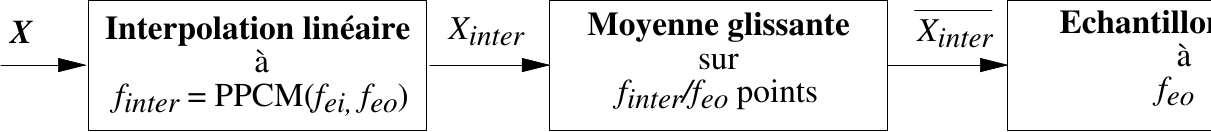
\includegraphics[width=0.8\linewidth]{images/algo_MoyEch_ff.png}
\captionof{figure}{Sch�ma fonctionnel de \operfmt{MoyEch\_ff}}
\label{fig:algo_MoyEch_ff}
}

%%%%%AUTEUR%%%%
\itemstyle{Auteur~:}
CNRM/GMEI/TRAMM

%%%%%REFERENCE%%%%
\itemstyle{R�f�rences~:}
